\documentclass{book}

% ======== Packages ========
\usepackage[a4paper, top=2cm, bottom=3cm, left=2.5cm, right=2.5cm]{geometry}
\usepackage{titlesec}
\usepackage{amsmath}
\usepackage{amsfonts}
\usepackage{amssymb}
\usepackage{tikz}
\usepackage{array}
\usepackage{xcolor}
\usepackage{etoolbox}
\usepackage[hidelinks]{hyperref}
\usepackage{lipsum}
\usepackage{lettrine}
\usepackage{listings}
\usepackage{inconsolata}
\usetikzlibrary{positioning, arrows.meta, shapes.geometric}

% ======== Custom Drop Cap Font (Zallman) ========
\usepackage{filecontents}
\begin{filecontents*}{Zallman.sty}
  \NeedsTeXFormat{LaTeX2e}
  \ProvidesPackage{Zallman}[2007/11/24 v1.0 Zallman CFR]
  \input Zallman.fd
  \DeclareRobustCommand{\Zallmanfamily}{
    \fontencoding{U}%
    \fontseries{xl}%
    \fontshape{n}%
    \fontfamily{Zallman}%
    \selectfont}
  \DeclareTextFontCommand{\zall}{\Zallmanfamily}
  \endinput
\end{filecontents*}
\usepackage{Zallman}
\renewcommand{\LettrineFontHook}{\color{Maroon}\Zallmanfamily}

% ======== Colors ========
\definecolor{deepred}{RGB}{153, 0, 0}
\definecolor{codebg}{RGB}{240,240,240}
\definecolor{codeborder}{RGB}{200,200,200}
\definecolor{keywordcolor}{RGB}{153, 0, 0}
\definecolor{Maroon}{RGB}{128, 0, 0}

% ======== Code Style ========
\lstdefinestyle{mystyle}{
  backgroundcolor=\color{codebg},
  basicstyle=\ttfamily\footnotesize,
  frame=single,
  rulecolor=\color{codeborder},
  keywordstyle=\color{keywordcolor}\bfseries,
  commentstyle=\color{gray},
  stringstyle=\color{blue},
  showstringspaces=false,
  breaklines=true,
  language=Python
}

% ======== Chapter spacing tweak ========
\makeatletter
\patchcmd{\@makechapterhead}{\vspace*{50\p@}}{\vspace*{10pt}}{}{}
\makeatother

% ======== Chapter style ========
\titleformat{\chapter}[display]
  {\normalfont\Large\bfseries}
  {\begin{tikzpicture}
      \fill[deepred] (0,0) rectangle (2,-2.8);
      \node[text=white, font=\small\bfseries, anchor=base] at (1,-0.3) {CHAPTER};
      \node[text=white, font=\fontsize{30}{36}\selectfont\bfseries] at (1,-1.5) {\thechapter};
    \end{tikzpicture}}
  {0.5em}
  {\MakeUppercase}
  [\vspace{0.3em}
   \small\itshape\mdseries\raggedleft
   "The true logic of this world is in the calculus of probabilities." \\
   \rule{\linewidth}{0.4pt} \\
   \textbf{--- James C. Maxwell}]
\titlespacing*{\chapter}{0pt}{0pt}{2em}

\titleformat{\section}
  {\normalfont\bfseries}
  {\thesection}
  {1em}{}

\titleformat{\subsection}
  {\normalfont\bfseries}
  {\thesubsection}
  {1em}{}

\newcolumntype{L}[1]{>{\raggedright\arraybackslash}p{#1}}
\newcolumntype{R}[1]{>{\raggedleft\arraybackslash}p{#1}}

% ======== Document starts ========
\begin{document}

% === COVER PAGE ===
\begin{titlepage}
\centering
\vspace*{3cm}
{\Huge\bfseries DEEP THINKING\par}
\vspace{0.5cm}
{\Large\itshape Notes on Learning Machines and the Human Mind\par}
\vspace{2cm}
{\LARGE\scshape Fauzy Madani\par}
\vfill
{\Large SMK Negeri 1 Garut \\ \texttt{fauzy\_madani@smknegeri1garut.sch.id}}
\vspace*{2cm}


\begin{tikzpicture}
  \draw[deepred, very thick] (0,0) rectangle (12,16);
  \node[anchor=south west, inner sep=0] (coverimg) at (0,0)
    {\includegraphics[width=12cm,height=16cm]{example-image}};
  \fill[white,opacity=0.8] (0,0) rectangle (12,16);
\end{tikzpicture}
\end{titlepage}
\clearpage

% === Author Page ===
\chapter*{About the Author}
\addcontentsline{toc}{chapter}{About the Author}

\vspace{2em}

\newcommand{\HRule}{\rule{\linewidth}{0.5mm}}

\begin{center}
  \textsc{\LARGE SMKN 1 Garut}\\[1.5cm] % Institution / school
  
  \textsc{\Large Cloud Computing and Web Development Enthusiast}\\[0.5cm] % Major heading
  
  \textsc{\large About the Author}\\[0.5cm] % Minor heading (optional)
  
  \HRule\\[0.4cm]
  
  {\huge\bfseries Fauzy Madani}\\[0.4cm] % Large name
  
  \HRule\\[1.5cm]
\end{center}

\noindent
\begin{minipage}{0.48\textwidth}
  \large
  \textit{Contact}\\
  \texttt{github.com/fauzymadani} \\
  \texttt{fauzy@example.com}
\end{minipage}
\hfill
\begin{minipage}{0.48\textwidth}
  \large
  \textit{Areas of Interest}\\
  \begin{itemize}
    \setlength\itemsep{0.6em}
    \item Linux and Open Source Systems
    \item Cloud Infrastructure (AWS, Debian-based servers)
    \item Programming (Python, Bash, PHP)
    \item Machine Learning and Data Science
    \item Internet Privacy and Cryptography
  \end{itemize}
\end{minipage}

\vfill

\begin{center}
  {\large \today} % date, you can replace with fixed date if you want
\end{center}

\vspace{2em}

\noindent Fauzy Madani is a student at SMKN 1 Garut, passionate about cloud computing and web development. He actively explores open-source systems, Linux server administration, and secure web development.

His interests also include the intersection of machine learning and human cognition, with experiments in neural networks and data visualization. Fauzy shares his projects on GitHub and participates in various technology competitions, including Cloud Computing contests (LKS).

His long-term goal is to become a Debian package maintainer and contribute to reliable, privacy-focused software for the global community.

\clearpage

% === Continue with Table of Contents and next chapter ===
\tableofcontents
\clearpage

\chapter{How to Use This Book}
% === Table of Contents ===
\tableofcontents
\clearpage

% === CHAPTER 1 ===
\chapter{How to Use This Book}

% Illustration
\begin{center}
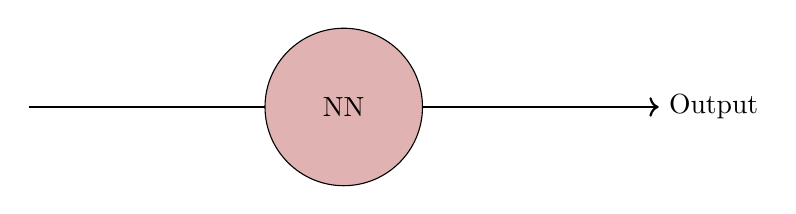
\begin{tikzpicture}
  \draw[->, thick] (0,0) -- (4,0) node[anchor=west] {Input};
  \draw[->, thick] (4,0) -- (8,0) node[anchor=west] {Output};
  \draw[fill=deepred!30] (4,0) circle (1);
  \node at (4,0) {NN};
\end{tikzpicture}

\vspace{0.5cm}
{\itshape Visual representation of a simple neural network.}
\end{center}

\section{Introduction}
\lettrine{F}{ irst of all}, involves carefully examining ideas beyond their surface level by systematically analyzing relationships, causes, and implications. It requires going beyond just accepting information as it is, instead questioning assumptions and exploring multiple layers of reasoning to understand the underlying principles. This kind of thinking uses formal logical processes like deduction and induction to draw well-founded conclusions and often involves breaking down complex problems into smaller, more manageable parts to analyze them thoroughly. From a technological standpoint, deep thinking means understanding how different parts of a system interact and affect each other, rather than looking at components in isolation. It involves creating solutions that are efficient, scalable, and robust by anticipating potential problems and edge cases. Technological deep thinking also requires a mindset of careful design — building abstractions and modular structures that manage complexity while maintaining flexibility. This means thinking not only about how something works right now but also how it will behave under different conditions or how it can be adapted in the future. Essentially, deep thinking in both realms is about moving beyond superficial understanding to grasp the intricate details and bigger picture simultaneously, enabling better decision-making and problem-solving.

\subsection{What makes this book so valuable}
\lettrine{D}{ eciphering} dead languages. Detecting malignant tumours. develop a skill that’s crucial but often overlooked: the ability to analyze complex problems thoughtfully and thoroughly. In today’s fast-paced world, many people tend to skim information or jump to quick conclusions, but deep thinking encourages slowing down, questioning assumptions, and understanding systems at a fundamental level. Such a book would provide practical frameworks and mental tools to approach challenges more effectively, whether in everyday life, science, engineering, or technology. It can also bridge the gap between abstract reasoning and real-world application, helping readers not just to think harder but to think smarter—anticipating problems, designing better solutions, and making decisions that stand the test of time. Ultimately, its value lies in empowering readers to cultivate clarity, insight, and creativity, which are essential for innovation and meaningful progress in any field.

% === CHAPTER 2 ===
\chapter{Deep Learning Basics}

\section{What is a Neural Network?}
\lettrine{A}{ rtificial} type of computational model inspired by the way biological brains work, designed to recognize patterns and solve complex problems by learning from data. At its core, a neural network is composed of many interconnected units called neurons or nodes, arranged in layers. These layers typically include an input layer, one or more hidden layers, and an output layer.
Each neuron receives input signals (which are usually numbers) from neurons in the previous layer, processes them by applying a weighted sum followed by a non-linear function called an activation function, and then passes the result to neurons in the next layer. The weights represent the strength or importance of the connections, and the activation function introduces non-linearity, enabling the network to model complex relationships rather than just linear ones.
Training a neural network involves adjusting these weights so that the network’s output matches the desired output as closely as possible. This is done through a process called backpropagation combined with an optimization algorithm like gradient descent. Backpropagation works by calculating the error between the predicted output and the actual output, then propagating this error backward through the network to update the weights in a way that reduces the error over time.
Neural networks are particularly powerful because they can automatically learn representations from raw data without needing explicit feature engineering. For example, in image recognition, early layers might detect simple features like edges, while deeper layers identify more complex shapes or objects.
There are many types of neural networks designed for specific tasks. For instance, feedforward neural networks process data in one direction from input to output, while recurrent neural networks (RNNs) have loops allowing them to process sequences and remember past information, which is useful in language processing. Another type, convolutional neural networks (CNNs), uses specialized layers to efficiently analyze visual data.
Overall, neural networks form the backbone of many modern AI applications, including speech recognition, natural language processing, autonomous driving, and more, because of their ability to learn complex patterns and generalize well to new, unseen data.

\subsection{Perceptron}
\lettrine{T}{ he} perceptron is a binary classifier. perceptron is one of the simplest types of artificial neural networks and actually a foundational building block for more complex neural networks. It was introduced in the 1950s by Frank Rosenblatt.
A perceptron takes several input values, each multiplied by a weight that represents the importance of that input. Then, it sums all these weighted inputs and passes the result through an activation function, typically a step function that outputs either 0 or 1. This output represents the perceptron’s decision—like classifying data into one of two categories.
Mathematically, if you think of inputs as a vector xx and weights as ww, the perceptron computes:
$$ y = \text{activation}\left(\sum_{i=1}^n w_i x_i + b \right) $$
where bb is a bias term that shifts the decision boundary.
The perceptron learns by adjusting the weights based on errors between its predicted output and the actual target during training, using a simple update rule. While a single perceptron can only solve linearly separable problems (where a straight line can separate classes), stacking perceptrons and adding layers leads to more powerful models like multilayer neural networks that can learn complex patterns.
In short, the perceptron is the building block for neural networks, helping machines make simple yes/no decisions and forming the basis for deep learning architectures.

\section{Training the model}
\noindent
Training a model involves finding the right set of parameters (weights and biases) that minimize the error between the predicted output and the actual output. This process is essentially an optimization problem. The model "learns" by iteratively adjusting its parameters using algorithms like gradient descent. Over time, these adjustments improve the model's accuracy.
\begin{center}
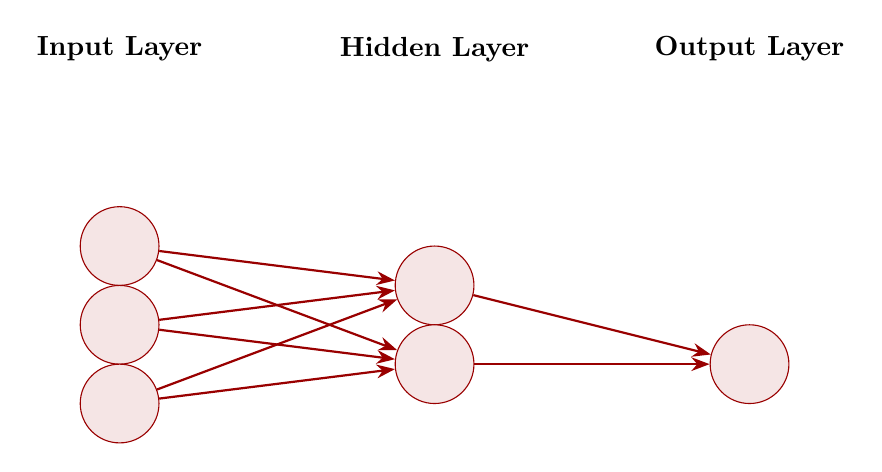
\begin{tikzpicture}[
  neuron/.style={circle, draw=deepred, fill=deepred!10, minimum size=1cm},
  layer/.style={draw=none, font=\bfseries},
  connection/.style={->, thick, >=Stealth, draw=deepred},
  node distance=1cm and 1.5cm
]
  % Layers
  \node[layer] at (0,3.5) {Input Layer};
  \node[layer] at (4,3.5) {Hidden Layer};
  \node[layer] at (8,3.5) {Output Layer};

  % Input neurons
  \foreach \i in {1,2,3} {
    \node[neuron] (i\i) at (0,2-\i) {};
  }

  % Hidden neurons
  \foreach \j in {1,2} {
    \node[neuron] (h\j) at (4,1.5-\j) {};
  }

  % Output neuron
  \node[neuron] (o1) at (8,-0.5) {};

  % Connections: Input -> Hidden
  \foreach \i in {1,2,3} {
    \foreach \j in {1,2} {
      \draw[connection] (i\i) -- (h\j);
    }
  }

  % Connections: Hidden -> Output
  \foreach \j in {1,2} {
    \draw[connection] (h\j) -- (o1);
  }
\end{tikzpicture}

\vspace{0.5em}
\textit{Figure: A basic neural network during training. Weights are updated to reduce prediction error.}
\end{center}

\subsection{Backpropagation}
\vspace{0.5em}
\noindent
To understand how errors propagate backward through layers, consider the basic gradient descent update rule:
\begin{equation}
  w := w - \eta \frac{\partial L}{\partial w}
\end{equation}

\noindent
Where:
\begin{itemize}
  \item \textit{\( w \)} is a weight parameter,
  \item \textit{\( \eta \)} is the learning rate,
  \item \textit{\( \frac{\partial L}{\partial w} \)} is the partial derivative of the loss function with respect to the weight.
\end{itemize}

\vspace{0.4em}
\begin{center}
  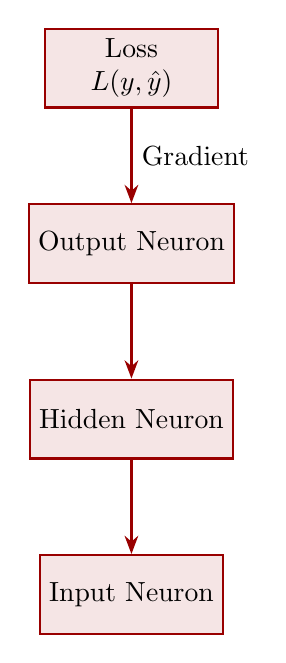
\begin{tikzpicture}[
    block/.style={
      rectangle,
      draw=deepred,
      thick,
      fill=deepred!10,
      minimum width=2.2cm,
      minimum height=1cm,
      align=center
    },
    arrow/.style={->, thick, >=Stealth, draw=deepred},
    node distance=1.2cm
  ]
    \node[block] (loss) {Loss \\ \( L(y, \hat{y}) \)};
    \node[block, below=of loss] (output) {Output Neuron};
    \node[block, below=of output] (hidden) {Hidden Neuron};
    \node[block, below=of hidden] (input) {Input Neuron};

    \draw[arrow] (loss) -- node[right] {Gradient} (output);
    \draw[arrow] (output) -- (hidden);
    \draw[arrow] (hidden) -- (input);
  \end{tikzpicture}

  \vspace{0.4em}
  \textit{Figure: Backpropagation through layers using gradient descent.}
\end{center}

\vspace{0.3em}
\noindent
Backpropagation efficiently applies the chain rule:
\begin{equation}
  \frac{\partial L}{\partial w} =
  \frac{\partial L}{\partial y} \cdot
  \frac{\partial y}{\partial z} \cdot
  \frac{\partial z}{\partial w}
\end{equation}

\noindent
Each term in this chain corresponds to a different layer in the network, enabling us to compute how much each weight contributes to the overall loss.

\lettrine{B}{ ackpropagation} is an essential technique. fundamental algorithm in AI and deep learning that enables neural networks to learn from data by adjusting their internal parameters—called weights—in order to improve performance on a given task. When a neural network processes an input, it produces an output, which is then compared to the expected or correct result using a loss function—a measure of how far off the prediction is. The goal of training is to minimize this loss.
Backpropagation works by computing the gradient, or the rate of change, of the loss function with respect to each weight in the network. This gradient tells us how much a small change in a particular weight will affect the overall error. The algorithm uses the chain rule from calculus to efficiently calculate these gradients layer by layer, starting from the output layer and moving backward toward the input layer—hence the name “backpropagation.”
Once the gradients are computed, they guide how the weights should be adjusted. Using an optimization method like gradient descent, the network updates its weights in the direction that most reduces the loss. This process repeats over many iterations (epochs), gradually improving the network’s accuracy in making predictions.
Without backpropagation, training deep neural networks would be extremely difficult because it allows the model to assign credit or blame to each connection based on its contribution to the final error, enabling the network to learn complex, multi-layered representations from data. This makes backpropagation a cornerstone technique that drives much of the progress in deep learning and modern AI applications.

% Complex Flowchart
\begin{center}
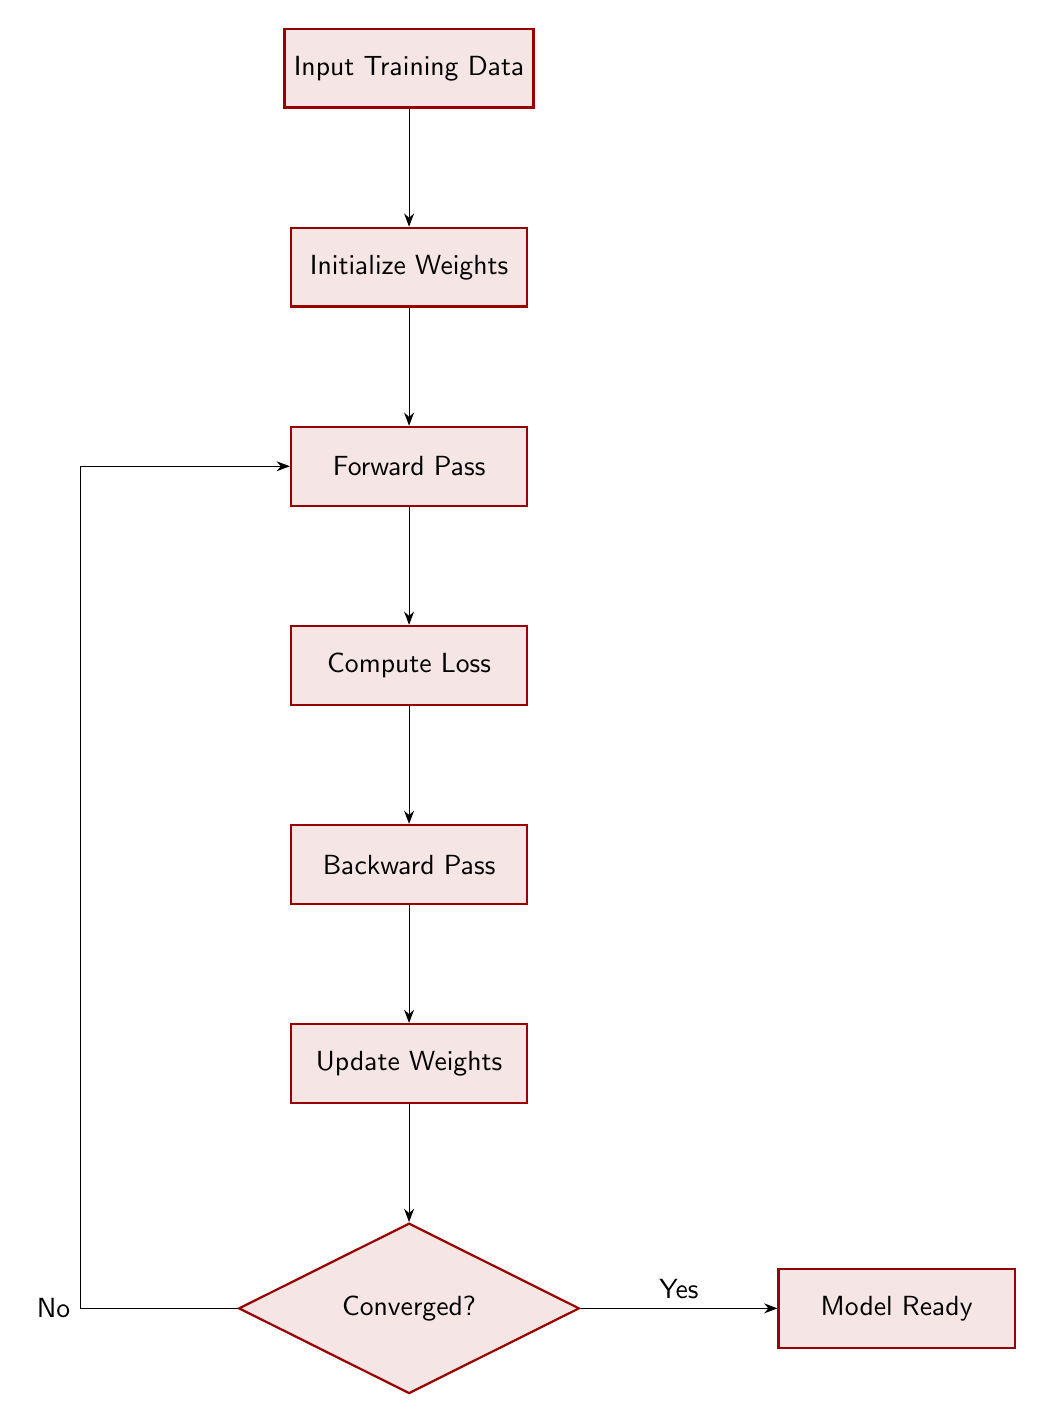
\begin{tikzpicture}[
  node distance=1.5cm and 2.5cm,
  every node/.style={font=\sffamily},
  process/.style={rectangle, draw=deepred, thick, fill=deepred!10, minimum width=3cm, minimum height=1cm},
  decision/.style={diamond, draw=deepred, thick, fill=deepred!10, aspect=2, text width=3cm, align=center},
  >=Stealth
]

\node[process] (data) {Input Training Data};
\node[process, below=of data] (init) {Initialize Weights};
\node[process, below=of init] (fwd) {Forward Pass};
\node[process, below=of fwd] (loss) {Compute Loss};
\node[process, below=of loss] (bwd) {Backward Pass};
\node[process, below=of bwd] (update) {Update Weights};
\node[decision, below=of update] (check) {Converged?};
\node[process, right=of check] (done) {Model Ready};

\draw[->] (data) -- (init);
\draw[->] (init) -- (fwd);
\draw[->] (fwd) -- (loss);
\draw[->] (loss) -- (bwd);
\draw[->] (bwd) -- (update);
\draw[->] (update) -- (check);
\draw[->] (check) -- node[above] {Yes} (done);
\draw[->] (check.west) -- ++(-2,0) node[left] {No} |- (fwd.west);

\end{tikzpicture}

\vspace{0.5cm}
{\itshape A more detailed training loop in a deep learning pipeline.}
\end{center}

\begin{lstlisting}[style=mystyle, caption={A simple neural net in PyTorch}]
import torch
import torch.nn as nn

class Net(nn.Module):
    def __init__(self):
        super(Net, self).__init__()
        self.fc = nn.Linear(10, 1)

    def forward(self, x):
        return self.fc(x)
\end{lstlisting}

% === CHAPTER 3 ===
\chapter{Advanced Topics}

\section{GANs and VAEs}
\lettrine{G}{ enerative} models like GANs are powerful. Generative Adversarial Networks (GANs) are a class of neural networks designed to generate new, realistic data samples that resemble a given dataset. A GAN consists of two neural networks working in opposition—a generator and a discriminator. The generator creates fake data (like images, text, or audio) from random noise, trying to mimic the real data distribution. The discriminator’s job is to distinguish between real data (from the training set) and fake data produced by the generator. During training, these two networks play a kind of game: the generator tries to fool the discriminator by producing increasingly convincing fake samples, while the discriminator gets better at spotting fakes. Through this adversarial process, both networks improve over time. The end result is a generator that can produce highly realistic data. GANs have been widely used for tasks like image synthesis, style transfer, and even creating deepfake videos.
while Variational Autoencoders (VAEs), on the other hand, are a different kind of generative model that learns to encode input data into a compressed, continuous latent space and then decode it back to reconstruct the original input. Unlike traditional autoencoders, VAEs learn a probability distribution over the latent space rather than fixed points. This allows VAEs to generate new data by sampling from the latent space and decoding it. The key idea behind VAEs is to balance two objectives during training: minimizing the reconstruction error (how close the decoded output is to the original input) and ensuring the latent space follows a known distribution (usually a Gaussian). This makes the latent space smooth and continuous, which helps generate coherent new samples by interpolation. VAEs are often used in tasks such as image generation, anomaly detection, and representation learning. In summary, both GANs and VAEs are powerful generative models but work quite differently: GANs use a competitive training setup between two networks to produce realistic samples, while VAEs use probabilistic encoding and decoding to learn a meaningful latent representation that can be sampled for new data. Each has its own strengths and applications depending on the problem you want to solve.

% === CHAPTER 4 ===
\chapter{Interview Questions}

\section{Theory}
\lettrine{T}{ his} section covers theoretical concept. deep learning models combines ideas from mathematics and computer science: neural networks approximate complex functions by layering simple mathematical operations, and backpropagation uses calculus to efficiently adjust the network’s parameters to reduce errors. GANs rely on game theory, where two networks compete to generate realistic data by learning the true data distribution, while VAEs use principles from probability and Bayesian inference to learn compact, meaningful representations of data and generate new samples by balancing reconstruction accuracy with keeping the underlying data structure organized. Together, these theories enable machines to learn from data, recognize patterns, and create new content in powerful and flexible ways.

\section{Coding}
\lettrine{I}{ nterviewers} often ask you to write code. t’s their goal is to assess more than just whether you
can produce a working program. They want to see your problem-solving process, logical thinking,
and how you approach complex challenges step-by-step—which is essentially a form of deep thinking
applied in a practical context. Writing code live reveals how you break down problems, choose the right
algorithms or data structures, and handle edge cases or errors. It also shows your ability to communicate
your reasoning clearly and adapt when faced with unfamiliar scenarios. So, the coding task isn’t just
about getting the right answer; it’s about demonstrating your mindset, technical skills, and capacity to
think deeply and logically under pressure, which are critical traits for real-world software development.

\end{document}

